\section{Wyniki}
\subsection{Testy implementacji}

Głównym celem pracy było znalezienie rozwiązania problemu logarytmu dyskretnego
dla krzywej ECCp79 z Certicom Challenge w możliwie najkrótszym czasie. Mimo że
rozmiar krzywej jest stosunkowo niewielki, a współczesny sprzęt znacznie
wydajniejszy od tego dostępnego w momencie pierwszych prób złamania tej krzywej,
obliczenie rozwiązania wciąż zajmuje czas liczony w godzinach.

Ze względu na czasochłonność pełnych obliczeń, niezbędne było przeprowadzenie
testów implementacji na mniejszych, uproszczonych problemach, które pozwoliłyby
na szybszą weryfikację poprawności algorytmu i jego działania. Testy te były
niezbędnym krokiem przed przystąpieniem do pełnoprawnych prób rozwiązania
problemu logarytmu dyskretnego dla krzywej ECCp79. Pozwoliły one na upewnienie się,
że implementacja działa poprawnie oraz spełnia wszystkie założenia teoretyczne.

W tym celu wykorzystano środowiska PyTest oraz SageMath do przeprowadzenia testów
funkcjonalnych, weryfikujących poprawność operacji na krzywych eliptycznych
oraz pierwszych kroków algorytmu Rho Pollarda.

Testy obejmowały następujące aspekty:
\begin{itemize}
    \item Poprawność dodawania punktów na krzywej eliptycznej:
          Wyniki obliczeń programu klienta były porównywane z wynikami uzyskanymi
          w SageMath.
    \item Weryfikacja pierwszych kilkuset iteracji algorytmu Rho Pollarda:
          Sprawdzano zgodność wyników generowanych przez implementację z oczekiwanymi
          wartościami teoretycznymi.
    \item Sprawdzenie integralności przesyłanych danych pomiędzy serwerem a
          klientem: Testowano, czy format danych oraz zawartość są poprawnie przetwarzane
          na styku kodu Python'a oraz CUDA.
\end{itemize}

Wszystkie testy zostały pomyślnie zaliczone w obecnej wersji programu, co
potwierdza poprawność implementacji oraz zgodność wyników z teoretycznymi
oczekiwaniami.

\subsection{Wydajność}

W celu oceny wydajności implementacji program był wielokrotnie uruchamiany z
włączonym pełnym logowaniem każdego znalezionego punktu wyróżnionego. Wydajność
mierzono na podstawie przyrostu liczby znalezionych punktów w czasie, co pozwalało
na oszacowanie liczby iteracji dodawania punktów na sekundę.

Testy przeprowadzono przy założeniu, że punkt wyróżniony spełnia warunek 20
najmłodszych bitów współrzędnej $x$ równych $0$ w reprezentacji bitowej.
Sprawdzano sumę znalezionych punktów wyróżnionych w różnych odstępach czasu:
po 1 minucie oraz 5 minutach.

\begin{table}[h!]
    \centering
    \caption{Wyniki testów wydajności}
    \begin{tabular}{|c|c|c|}
        \hline
        \textbf{Czas testu} & \textbf{Liczba znalezionych punktów} &
        \textbf{Średnia liczba iteracji/s}                                \\ \hline
        1 minuta            & 5274                                 & 87.9 \\ \hline
        5 minut             & 26310                                & 87.7 \\ \hline
        % 10 minut            & <liczba punktów>                     & <wynik> \\ \hline
    \end{tabular}
    \label{tab:performance}
\end{table}

Na podstawie wyników testów oszacowano liczbę operacji dodawania punktów na
sekundę w algorytmie Rho Pollarda. Prawdopodobieństwo znalezienia punktu wyróżnionego,
gdy 20 najmłodszych bitów współrzędnej $x$ wynosi $0$, można określić jako
$$
    P = 2^{-20}.
$$

Średnia liczba iteracji potrzebna do znalezienia punktu wyróżnionego wynosi
więc:
$$
    \text{Średnia liczba iteracji} = \frac{1}{P} = 2^{20}.
$$

Na podstawie wyników testów, oszacowano, że implementacja osiąga wydajność na
poziomie 87,7 milionów operacji dodawania punktów na sekundę.

\subsection{Rozwiązanie ECDLP dla krzywej ECCp79}

Najważniejszym wyznacznikiem osiągnięcia założonego celu tej pracy było
znalezienie poprawnego rozwiązania ECDLP dla krzywej z challenge'u Certicom ECCp79.
Po zweryfikowaniu poprawności implementacji na znacznie mniejszych rozmiarach
krzywych eliptycznych, przystąpiłem do przeprowadzenia obliczeń dla docelowego
problemu. Proces ten wymagał wykonania dużej liczby iteracji algorytmu Rho Pollarda,
a jego wyniki zostały szczegółowo udokumentowane.

\begin{figure}[H]
    \centering
    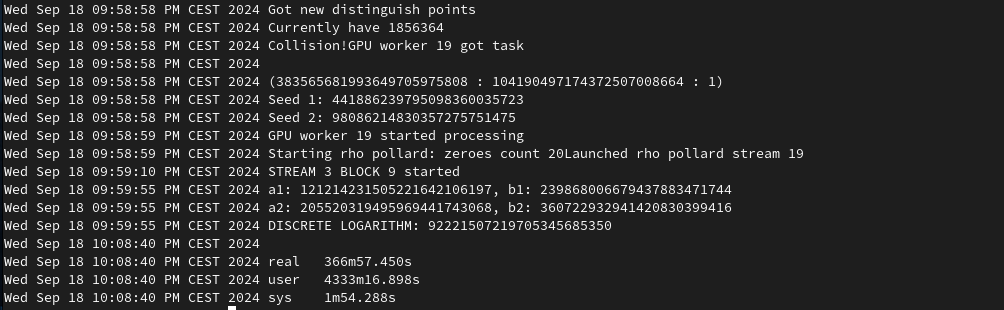
\includegraphics[width=0.8\textwidth]{img/first_attempt.png}
    \caption{Wynik działania programu}
    \label{fig:first_attempt}
\end{figure}

Poniżej przedstawiono wyniki pięciu niezależnych prób obliczenia ECDLP dla
krzywej ECCp79, wskazujące liczbę znalezionych punktów wyróżnionych do momentu
znalezienia kolizji oraz czas trwania obliczeń.

\begin{table}[H]
    \centering
    \caption{Wyniki obliczeń ECDLP dla krzywej ECCp79}
    \label{tab:eccp79_results}
    \begin{tabular}{|c|c|c|}
        \hline
        \textbf{Próba}   & \textbf{Liczba znalezionych punktów} &
        \textbf{Czas trwania obliczeń [s]}                                      \\ \hline
        1                & 1856364                             & 22195.42      \\ \hline
        2                & 791747                              & 9898.74       \\ \hline
        3                & 770077                              & 9329.74       \\ \hline
        4                & 1163047                             & 13681.16      \\ \hline
        5                & 1207014                             & 15001.94      \\ \hline
        \textbf{Średnia} & 1153649                             & 14021.00      \\ \hline
    \end{tabular}
\end{table}



\paragraph{Weryfikacja wyników za pomocą SageMath.}
Aby upewnić się, że uzyskane rozwiązanie ECDLP jest poprawne, przeprowadzono
weryfikację przy użyciu oprogramowania SageMath. Weryfikacja polegała na
podstawieniu uzyskanego wyniku logarytmu dyskretnego do równania punktowego
na krzywej eliptycznej i sprawdzeniu, czy generuje on punkt publiczny
zgodny z założeniami challenge'u Certicom ECCp79.

\begin{figure}[H]
    \centering
    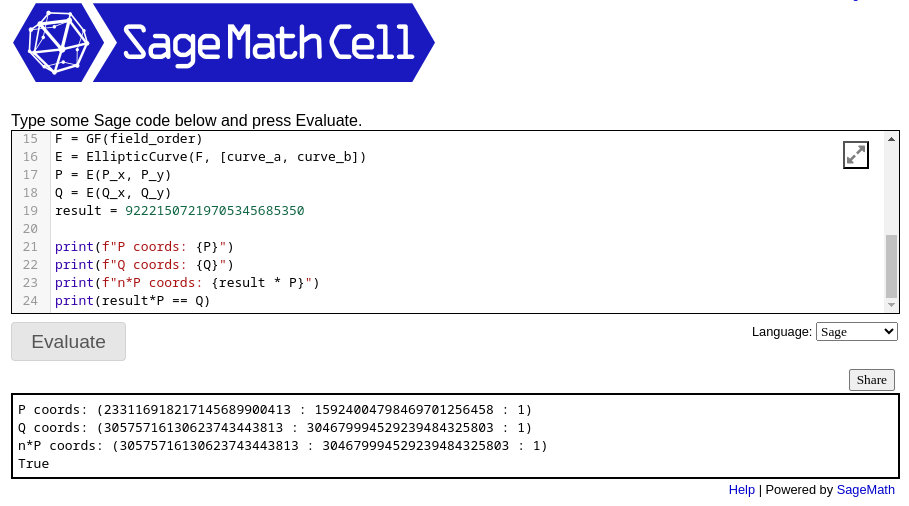
\includegraphics[width=0.8\textwidth]{img/sage_check_full.png}
    \caption{Weryfikacja wyniku w SageMath}
    \label{fig:sage_verification}
\end{figure}

Weryfikacja potwierdziła poprawność uzyskanego wyniku, co dowodzi skuteczności
implementacji oraz poprawności algorytmu w zastosowaniu do krzywej ECCp79.

\paragraph{Podsumowanie wyników.}
Na podstawie powyższych wyników można obliczyć średnią liczbę punktów wyróżnionych
znajdowanych przed wystąpieniem kolizji.
Porównanie wyniku z oczekiwanymi wartościami teoretycznymi, pozwoliło potwierdzić
osiągnięcie odpowiedniej losowości przy obliczaniu kolejnych kroków algorytmu.
Oczekiwaną liczbę punktów do znalezienia kolizji można oszacować na podstawie wzoru:
$$
    E = \frac{\sqrt{\pi \cdot n / 2}}{2^k}
$$
gdzie $n$ to liczność grupy punktów na krzywej eliptycznej, a $k$ to liczba bitów zerowych które decydują
czy dany punkt jest wyróżniony. W przypadku krzywej ECCp79,
dla $n \approx 2^{79}$, oraz punktów wyróżnionych których ostatnie 20 bitów to $0$, oczekiwana liczba
punktów potrzebna do znalezienia kolizji:
$$
    \frac{\sqrt{\pi \cdot 2^{79} / 2}}{2^{20}} = 929262.5811
$$
Uzyskany wynik na poziomie 1153649 jest bliski wartości oczekiwanej. Rozbieżność może wynikać z niewielkiej
liczby przeprowadzonych prób oraz ograniczonej liczby punktów wstępnie obliczonych.
Wydajność obliczeń jest zgodna z wynikami otrzymanymi podczas testów wydajności na ograniczonej liczbie iteracji algorytmu.
Najszybsze znalezienie logarytmu dyskretnego zajeło mniej niż 3 godziny, co jest bardzo zadowalającym wynikiem.